% =============================================================================
% TEST FIGURE - Protein Folding Performance Comparison
% =============================================================================
% This is a test figure created with TikZ
% You can replace this with your actual figures
% =============================================================================

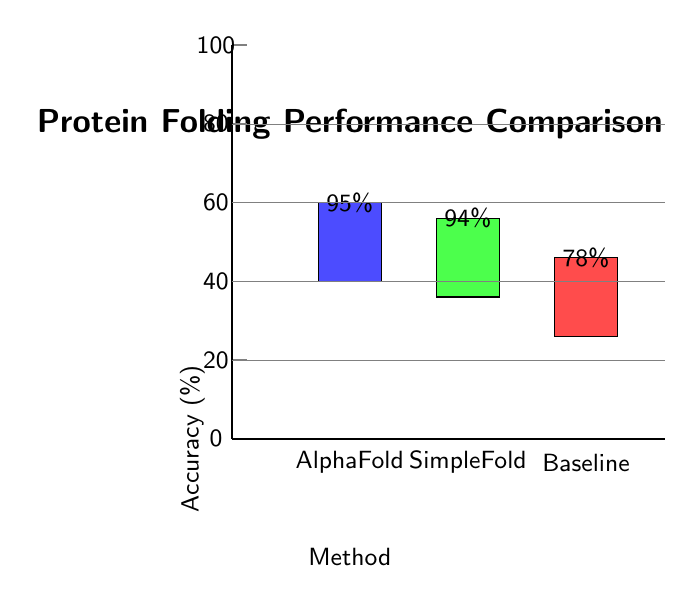
\begin{tikzpicture}
% Define styles
\tikzset{
    bar/.style={rectangle, draw=black, fill=blue!50, minimum height=1cm, minimum width=0.8cm},
    label/.style={font=\small\sffamily},
    title/.style={font=\large\bfseries\sffamily}
}

% Title
\node[title] at (0, 4) {Protein Folding Performance Comparison};

% Y-axis label
\node[label, rotate=90] at (-2, 0) {Accuracy (\%)};

% X-axis label
\node[label] at (0, -1.5) {Method};

% Y-axis ticks and labels
\foreach \y/\label in {0/0, 1/20, 2/40, 3/60, 4/80, 5/100} {
    \draw[gray] (-1.5, \y) -- (-1.3, \y);
    \node[label] at (-1.7, \y) {\label};
}

% Y-axis line
\draw[thick] (-1.5, 0) -- (-1.5, 5);

% X-axis line
\draw[thick] (-1.5, 0) -- (4, 0);

% Bars
\node[bar, fill=blue!70] at (0, 2.5) {};
\node[label] at (0, -0.3) {AlphaFold};

\node[bar, fill=green!70] at (1.5, 2.3) {};
\node[label] at (1.5, -0.3) {SimpleFold};

\node[bar, fill=red!70] at (3, 1.8) {};
\node[label] at (3, -0.3) {Baseline};

% Values on top of bars
\node[label] at (0, 3) {95\%};
\node[label] at (1.5, 2.8) {94\%};
\node[label] at (3, 2.3) {78\%};

% Grid lines
\foreach \y in {1, 2, 3, 4} {
    \draw[gray, very thin] (-1.5, \y) -- (4, \y);
}

\end{tikzpicture}
